\section{Dataset}

All the data we will use in this project are from Github. There is not an existing complete dataset to get enough well-structured data for our project, so we need to collect data and preprocess by ourselves. In this section, we will illustrate why we choose Github's data and what the data sources are.

\subsection{Why Github}
Github is the largest developer community and the largest platform for developers to share their codes and collaborate with others in the world. By analyzing the data from Github, we can get some insights about the development of open source projects, the development of programming languages, and the development of the developer community.



\subsection{Source I: Open API}
Github provides a series of open API for developers to access most of the informations on Github. This 'Github REST API\cite{ghapi}' is mainly used for creating integrations, retrieve data, and automate workflows, but we can use it to query specific data needed for our project.

There are mainly two main areas of data:

\begin{itemize}
    \item \textbf{Users:} Basic open informations of user, such as id, name, email, following users, repositories owned, etc.
    \item \textbf{repositories:} Basic information of public repositories, such as id, name, owner, description, stars etc.
\end{itemize}

We will provide some examples results of API query in Appendix\ref{a-ghrest}.

There are limits of current official REST API:
\begin{itemize}
    \item Some need authentication, which means we need to provide a valid token to access the data.
    \item Some API cannot be called too frequently, which means we need to wait for a while before we can call it again.
    \item Most of API need an \textbf{\textit{id}} as its query parameter, so we need to get the id first before we can query the data, which means we need to construct a massive id list.
\end{itemize}

After considering the above limitations, we decide to use the Github Archive\cite{gha} as our main data source and use the REST API to get some additional data or search some specific content.


\subsection{Source II: Github Archive}

\textit{GH Archive\cite{gha} is a project to record the public GitHub timeline, archive it, and make it easily accessible for further analysis.} In fact, it also based on Github's Open API, while only use the \textbf{activity} API:



\begin{minted}[breaklines,breakautoindent,mathescape,linenos,numbersep=1pt,frame=lines,framesep=2mm,fontsize=\footnotesize,baselinestretch =1,style=emacs]{python}
    https://api.github.com/events
\end{minted}


\textbf{GH Archive} will crawl github's activity data in real time and sort them as json file in order of when they occurred. Activity archives are available starting from 2011-02-12, and are updated amost half day, so the total size of data is \textbf{TB} level. 

Considering too large size of the data and the the earlist data using a different format, we will only use the latest part of them. In fact, the current amount data of data in an hour is about 700MB, so the latest data is surely enough for our project. The corresponding compression packages with specific time can be downloaded easily, and the minimal time interval of packages is one hour. 

\begin{figure}[H]
    \centering
    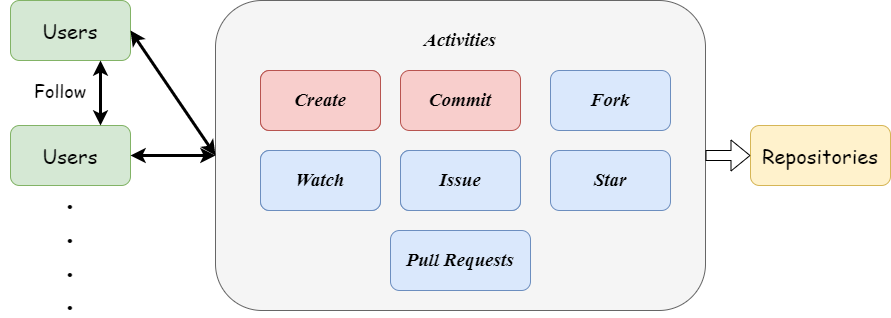
\includegraphics[width=0.52\textwidth]{./pic/github.png}
    \caption{This figure shows relation between user and repository and basic activities.}
    \label{fig:github}
\end{figure}


The archieved activity data contains almost all 20+ event types provided by Github, which ranges from new commits and fork events, to adding members to a project. We will only pay attention to some key event type, such as \textit{commit}, \textit{create}, etc.

We will give some example of the data format in Appendix\ref{a-gha}.


\subsection{Summary}
Based on almost all activity record, Github's Open API can help us to get almost all related information. For example, from \textbf{GH archive}, we know user a push a commit at 12:00 in repository A, then we can get almost all details of a and A by calling Github's API.






